\section{Software and supplementary examples}
\label{app:artifacts}

\subsection{Software versions}
\label{app:software-versions}
The inspected Codex CLI installation is version \texttt{0.155.1}
\citep{openai-codex}. Its upstream release tag \texttt{rust-v0.155.1} resolves to
commit \texttt{be2951ea34f0d295ed0becf97079f92fa5f6950e}.

The saved run configurations record the executable path but do not record its
version or binary hash; the installation was checked on 25 September 2026.
% EDITING NOTE: Do not assert that every historical run used this release without
% contemporaneous version evidence. See SOFTWARE_PROVENANCE.md for local evidence.

\subsection{Breadth-first search analysis}
\label{app:bfs-analysis}
\label{sec:exp-baselines}
\label{sec:results-baseline}

The saved BFS evaluation contains 725 attempts: 366/669 solved on easy samples
(54.7\%), 1/40 on medium, and 0/16 on hard. These attempts include repeated samples
and different budgets and are not paired with the recent ten-sample ablations.
BFS uses wall-clock, state-expansion, and depth limits, while model runs use turn
and call-timeout limits.
% Source: workspace/RESULTS/results.md.

A fold is specified by a line in current-plane coordinates together with a layer selection, and
both are drawn from small finite sets. Candidate lines are read off the crease pattern itself: the distinct lines through its mountain and valley edges,
carried forward through each distinct face transform into current coordinates, then deduplicated.
On a box-pleated pattern thousands of crease edges collapse to a few dozen lines. Layer selections
are not arbitrary subsets either, because a partial fold must be a contiguous run at one extremity
of the stack; the selections are the whole stack, the top $k$, and the bottom $k$, which is about
$2N$ for $N$ layers rather than $2^N$, with the over or under direction forced for partials. Each
surviving candidate is judged by the same function the \texttt{add\_fold} tool calls, so a listed
fold cannot be one the tool would then reject, and it is dropped if it fails any material check of
Section~\ref{sec:env-refusals} or would crease the sheet where the target pattern carries no
crease.

Across 73,750 enumerations recorded in the saved runs, this evaluates a mean of about 2,010
candidate actions per state and returns 3.51 of them, a ratio of approximately 570 between evaluated and returned candidates.
The baseline expands with the same enumerator the model is given, tests goals with the
same terminal comparator that decides \texttt{solved}, reads no reference sequence, and runs under
a per-sample wall-clock budget with caps on states expanded and depth.

% Included by sections/appendix-bfs.tex. Regenerate with
%   node workspace/figures/make_depth_wall_figure.mjs \
%     --data workspace/depth_wall/depth_wall.csv --enum workspace/enum_cost/enum_cost.json
% then copy workspace/figures/out/depth_wall.tex here and drop the standalone wrapper.
\begin{figure}[t]
\centering
% BFS depth wall, one curve per tier.
% Cost model: t(d) = b^d * c0 * g^d, with the per-node enumeration cost measured
% Generated by workspace/figures/make_depth_wall_figure.mjs
% Source: workspace/depth_wall/depth_wall.csv
% easy: b = 2.721, g = 1.441, c0 = 4.26e-3s (b*g = 3.92, 14 profiled states), reference depth 6.8, predicted 46 s (b fitted on 7 budget-exhausted runs over 3 samples)
% mid: b = 3.147, g = 1.472, c0 = 1.49e-2s (b*g = 4.63, 11 profiled states), reference depth 12.0, predicted 17 d (b fitted on 12 budget-exhausted runs over 3 samples)
% hard: b = 7.050, g = 1.758, c0 = 3.18e-1s (b*g = 12.39, 12 profiled states), reference depth 19.0, predicted 5.9e+12 y (b fitted on 8 budget-exhausted runs over 2 samples)
%
% Standalone: pdflatex depth_wall.tex
% In a paper: keep the tikzpicture, drop the documentclass wrapper.
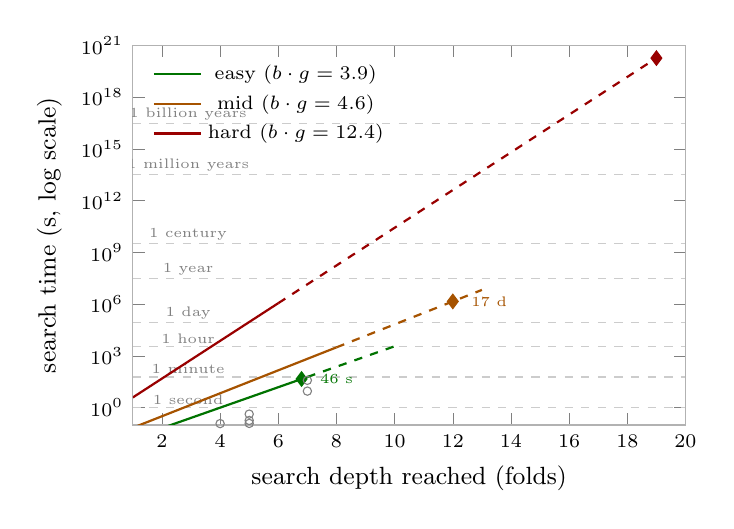
\begin{tikzpicture}
\begin{axis}[
  width=8.6cm, height=6.4cm,
  ymode=log,
  xlabel={search depth reached (folds)},
  ylabel={search time (s, log scale)},
  xmin=1, xmax=20, ymin=1e-1, ymax=1e21,
  xtick={2,4,6,8,10,12,14,16,18,20},
  ytick={1e0,1e3,1e6,1e9,1e12,1e15,1e18,1e21},
  tick label style={font=\scriptsize},
  label style={font=\small},
  legend style={font=\scriptsize, at={(0.02,0.98)}, anchor=north west, draw=none, fill=none},
  axis line style={gray!60},
]
\draw[gray!40, dashed, thin] (axis cs:1,1.0000e+0) -- (axis cs:20,1.0000e+0)
  node[pos=0.10, above, font=\tiny, gray, inner sep=1pt] {1 second};
\draw[gray!40, dashed, thin] (axis cs:1,6.0000e+1) -- (axis cs:20,6.0000e+1)
  node[pos=0.10, above, font=\tiny, gray, inner sep=1pt] {1 minute};
\draw[gray!40, dashed, thin] (axis cs:1,3.6000e+3) -- (axis cs:20,3.6000e+3)
  node[pos=0.10, above, font=\tiny, gray, inner sep=1pt] {1 hour};
\draw[gray!40, dashed, thin] (axis cs:1,8.6400e+4) -- (axis cs:20,8.6400e+4)
  node[pos=0.10, above, font=\tiny, gray, inner sep=1pt] {1 day};
\draw[gray!40, dashed, thin] (axis cs:1,3.1558e+7) -- (axis cs:20,3.1558e+7)
  node[pos=0.10, above, font=\tiny, gray, inner sep=1pt] {1 year};
\draw[gray!40, dashed, thin] (axis cs:1,3.1558e+9) -- (axis cs:20,3.1558e+9)
  node[pos=0.10, above, font=\tiny, gray, inner sep=1pt] {1 century};
\draw[gray!40, dashed, thin] (axis cs:1,3.1558e+13) -- (axis cs:20,3.1558e+13)
  node[pos=0.10, above, font=\tiny, gray, inner sep=1pt] {1 million years};
\draw[gray!40, dashed, thin] (axis cs:1,3.1558e+16) -- (axis cs:20,3.1558e+16)
  node[pos=0.10, above, font=\tiny, gray, inner sep=1pt] {1 billion years};
\addplot[thick, color=green!45!black, mark=none] coordinates {
  (1,1.66830e-2)
  (2,6.54005e-2)
  (3,2.56383e-1)
  (4,1.00507e+0)
  (5,3.94007e+0)
  (6,1.54458e+1)
  (7,6.05506e+1)
};
\addlegendentry{easy ($b\cdot g=3.9$)}
\addplot[thick, dashed, color=green!45!black, mark=none, forget plot] coordinates {
  (7,6.05506e+1)
  (8,2.37370e+2)
  (9,9.30537e+2)
  (10,3.64789e+3)
};
\addplot[thick, color=orange!65!black, mark=none] coordinates {
  (1,6.89243e-2)
  (2,3.19313e-1)
  (3,1.47932e+0)
  (4,6.85338e+0)
  (5,3.17504e+1)
  (6,1.47093e+2)
  (7,6.81456e+2)
  (8,3.15705e+3)
};
\addlegendentry{mid ($b\cdot g=4.6$)}
\addplot[thick, dashed, color=orange!65!black, mark=none, forget plot] coordinates {
  (8,3.15705e+3)
  (9,1.46260e+4)
  (10,6.77595e+4)
  (11,3.13917e+5)
  (12,1.45432e+6)
  (13,6.73756e+6)
};
\addplot[thick, color=red!60!black, mark=none] coordinates {
  (1,3.94464e+0)
  (2,4.88768e+1)
  (3,6.05619e+2)
  (4,7.50405e+3)
  (5,9.29805e+4)
  (6,1.15209e+6)
};
\addlegendentry{hard ($b\cdot g=12.4$)}
\addplot[thick, dashed, color=red!60!black, mark=none, forget plot] coordinates {
  (6,1.15209e+6)
  (7,1.42753e+7)
  (8,1.76881e+8)
  (9,2.19168e+9)
  (10,2.71564e+10)
  (11,3.36487e+11)
  (12,4.16932e+12)
  (13,5.16608e+13)
  (14,6.40114e+14)
  (15,7.93146e+15)
  (16,9.82765e+16)
  (17,1.21772e+18)
  (18,1.50884e+19)
  (19,1.86955e+20)
};
\addplot[only marks, mark=diamond*, mark size=2.6pt, color=green!45!black, forget plot]
  coordinates {(6.80,4.60741e+1)};
\node[font=\tiny, color=green!45!black, anchor=west] at (axis cs:7.10,4.60741e+1) {46 s};
\addplot[only marks, mark=diamond*, mark size=2.6pt, color=orange!65!black, forget plot]
  coordinates {(12.00,1.45432e+6)};
\node[font=\tiny, color=orange!65!black, anchor=west] at (axis cs:12.30,1.45432e+6) {17 d};
\addplot[only marks, mark=diamond*, mark size=2.6pt, color=red!60!black, forget plot]
  coordinates {(19.00,1.86955e+20)};

\addplot[only marks, mark=o, mark size=1.5pt, color=gray, forget plot] coordinates {
  (4,1.20000e-1)
  (5,4.25000e-1)
  (5,1.82000e-1)
  (5,1.23000e-1)
  (7,9.14900e+0)
  (7,3.87370e+1)
};
\end{axis}
\end{tikzpicture}
\caption{\textbf{Breadth-first search time against search depth, by difficulty group.}
The vertical axis is logarithmic, so a straight line is exponential growth and its slope is
$\log(b\cdot g)$. Curves are $t(d)=c_0(b\cdot g)^d$, the product of two exponentials: the
frontier grows as $b^d$ for a deduplicated branching factor $b$, measured as generated over
expanded during search, while the cost of expanding one node grows as $g^d$, because one
enumeration evaluates $4\times(\text{distinct crease lines})\times(\text{facets})$ candidates
and a fold of all layers at most doubles the facets. $g$ and $c_0$ are fitted by least squares
on per-depth enumeration timings. Each curve is solid only where that group was observed and
dashed beyond, and spans only the depths its own corpus reaches. Diamonds are each group's
mean reference depth; the hard group's sits at $10^{20}$ seconds, which is why the axis runs
that far. Circles are observed solves. $b$ is fitted from budget-exhausted runs: 7 over 3
samples for easy, 12 over 3 for medium, and 8 over 2 for hard, across 5 time budgets. The
hard extrapolation rests on two samples. Extrapolated values are model projections,
not measured solution times or lower bounds.}
\label{fig:depth-wall}
\end{figure}


The supplementary cost model approximates search time as the product of two exponential factors:
the frontier grows with the branching factor, and the cost of expanding one node grows with depth
as well, because one enumeration evaluates four candidates per crease line per facet and a fold of
all layers at most doubles the facets. Fitting both from the saved searches gives a per-fold
multiplier of 3.9 on the easy group, 4.6 on medium and 12.4 on hard
(Figure~\ref{fig:depth-wall}). These fitted curves extrapolate beyond the observed depths; they are not measured
solution times or lower bounds. The hard-group fit uses only two samples.
% EDITING NOTE: Validate the cost model and extrapolations before submission.


% Source: workspace/RESULTS/results.md, Deterministic search baseline.
% Static TeX bars; no additional plotting package or runtime required.
\begin{figure}[t]
\centering
\small
\begin{tabular}{llr}
Stratum (reference folds) & Median states expanded & Solved / attempts \\
\hline
Easy (4--10) & \rule{0.247cm}{8pt}\quad 65 & 366/669 \\
Medium (11--13) & \rule{4cm}{8pt}\quad 1,051.5 & 1/40 \\
Hard (14--19) & \rule{2.024cm}{8pt}\quad 532 & 0/16 \\
\end{tabular}
\caption{Observed BFS search effort in the saved aggregate. Bar lengths use a linear scale and
show median states expanded across attempts, including unsuccessful attempts. Budgets and repeated
samples are not standardized by this aggregate; 358 of 725 attempts terminated in timeout.
The lower hard-stratum median does not imply that hard instances require less search.
Reference depth is not minimum solution length.}
\label{fig:bfs-effort}
\end{figure}



\subsection{Dataset generation}
\label{app:generation-procedure}

{\small\begin{verbatim}
GENERATE(reference_depth, action_model):
    state <- unfolded square
    actions, frames <- [], []
    for step in 1..reference_depth:
        candidates <- LEGAL_FOLDS(state, action_model)
        if candidates is empty: return FAILED
        action <- SAMPLE(candidates)
        state <- APPLY(state, action)
        actions.append(action)
        frames.append(state)
    cp <- CREASE_PATTERN_IN_ORIGINAL_SHEET(state)
    cp <- SPLIT_EDGES_AT_INTERSECTIONS(cp)
    if not REPLAY_CHECK(cp, actions, state): return FAILED
    return (cp, state, actions, frames, METADATA(actions))
\end{verbatim}}

\subsection{Evaluation pipeline}
\label{app:evaluation-pipeline}

{\small\begin{verbatim}
EPISODE(sample, model, condition, query_budget):
    cp, target <- LOAD_INPUTS(sample)
    session <- INITIALIZE(cp, target, unfolded_square)
    history <- []
    for query in 1..query_budget:
        obs <- OBSERVE(session, condition)
        call <- model(cp, target, obs, history, condition)
        if call is finish: break
        # Edits: add/remove fold, go to step, restore revision.
        # Reads: state, images, candidates, target feedback.
        result <- DISPATCH_TRANSACTIONALLY(session, call)
        # Rejected edits leave session unchanged but consume a query.
        # Read calls consume a query without changing the sequence.
        history.append(call, result)
        if STOPPING_RULE(session, history): break
    return SCORE(REPLAY(session.actions), REFERENCE_AT_SCORING(sample))
\end{verbatim}
}

\begin{figure}[t]
\centering
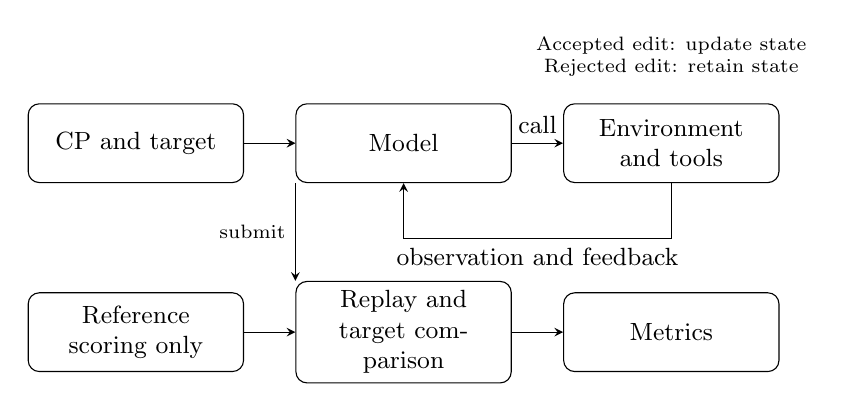
\begin{tikzpicture}[font=\small,box/.style={draw,rounded corners,align=center,text width=2.5cm,minimum height=1cm},>=stealth]
\node[box] (input) at (0,0) {CP and target};
\node[box] (model) at (3.4,0) {Model};
\node[box] (env) at (6.8,0) {Environment\\and tools};
\draw[->] (input)--(model);
\draw[->] (model)--node[above]{call}(env);
\draw[->] (env.south) -- ++(0,-.7) -| node[pos=.25,below]{observation and feedback}(model.south);
\node[align=center,font=\scriptsize] at (6.8,1.1) {Accepted edit: update state\\Rejected edit: retain state};
\node[box] (score) at (3.4,-2.4) {Replay and\\target comparison};
\node[box] (ref) at (0,-2.4) {Reference\\scoring only};
\node[box] (metrics) at (6.8,-2.4) {Metrics};
\draw[->] (model.south west)--node[left,font=\scriptsize]{submit}(score.north west);
\draw[->] (ref)--(score);
\draw[->] (score)--(metrics);
\end{tikzpicture}
\caption{Evaluation pipeline. The model edits and inspects its current construction. The reference
sequence is withheld from the model and used only for scoring.}
\label{fig:pipeline}
\end{figure}


\subsection{Tool schemas and prompt}
The following listings document the tool schemas and folding prompt; tool exposure is configured per run.
{\scriptsize\verbatiminput{../../DHEERAJ_WORKSPACE/EXPERIMENT_SETUP/tool_schemas.py}}
{\small\verbatiminput{../../DHEERAJ_WORKSPACE/EXPERIMENT_SETUP/fold_prompt.md}}

\subsection{Dataset gallery and reference sequences}
Each rendered panel contains the crease pattern, top view, and an oblique view with illustrative
layer separation.
\IfFileExists{figures/dataset/gallery.tex}{\noindent all-layers/easy-0001 (all-layers, 4 reference folds)\par
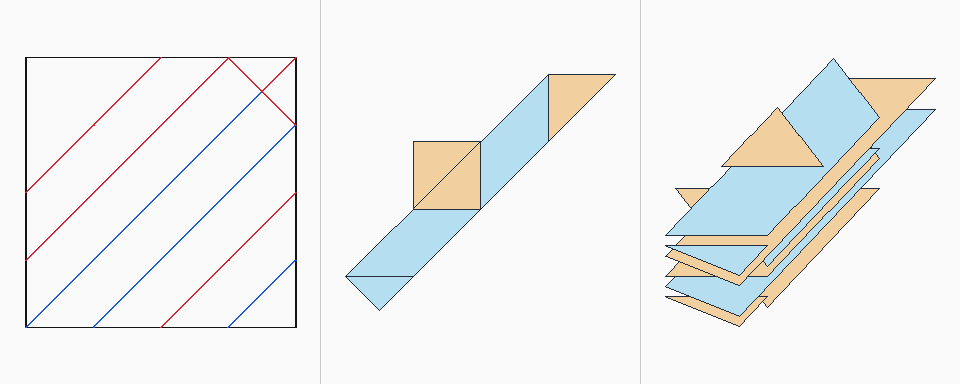
\includegraphics[width=\linewidth]{figures/dataset/sample-1.png}\par\medskip
\noindent all-layers/mid-0004 (all-layers, 11 reference folds)\par
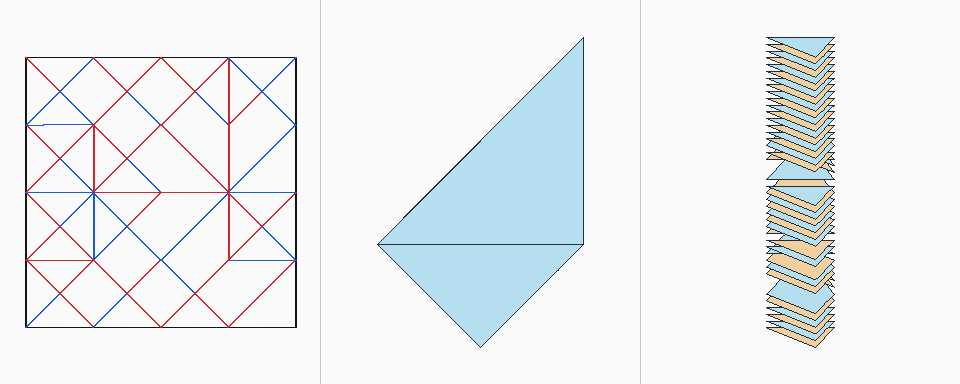
\includegraphics[width=\linewidth]{figures/dataset/sample-2.png}\par\medskip
\noindent some-generated-d5/layers-0001 (some-layers, 5 reference folds)\par
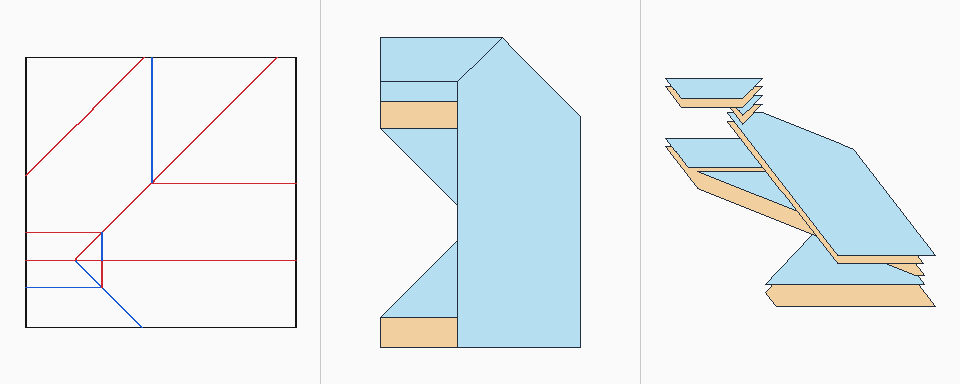
\includegraphics[width=\linewidth]{figures/dataset/sample-3.png}\par\medskip
\noindent all-layers/hard-0004 (all-layers, 15 reference folds)\par
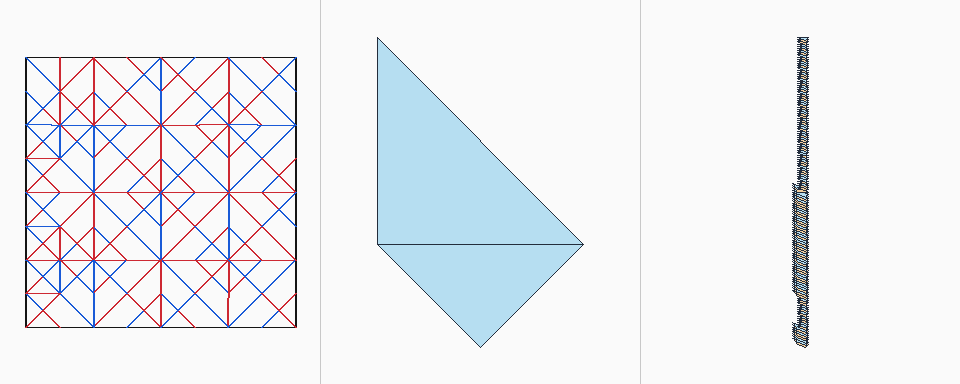
\includegraphics[width=\linewidth]{figures/dataset/sample-4.png}\par\medskip
\noindent all-layers/hard-0005 (all-layers, 15 reference folds)\par
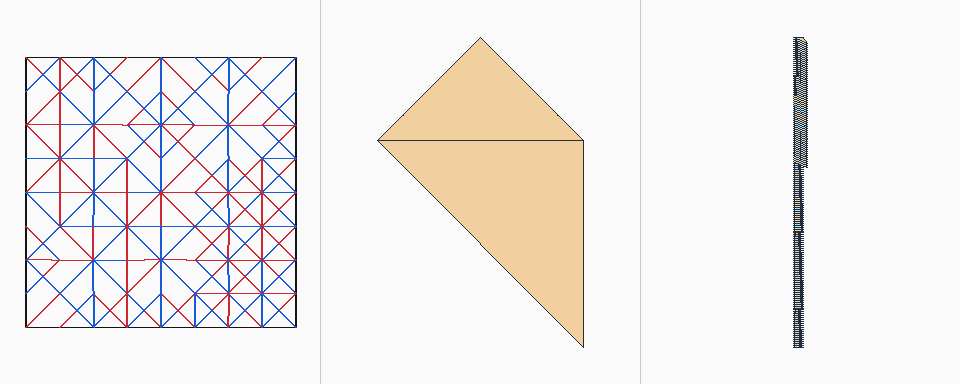
\includegraphics[width=\linewidth]{figures/dataset/sample-5.png}\par\medskip
\noindent all-layers/hard-0006 (all-layers, 15 reference folds)\par
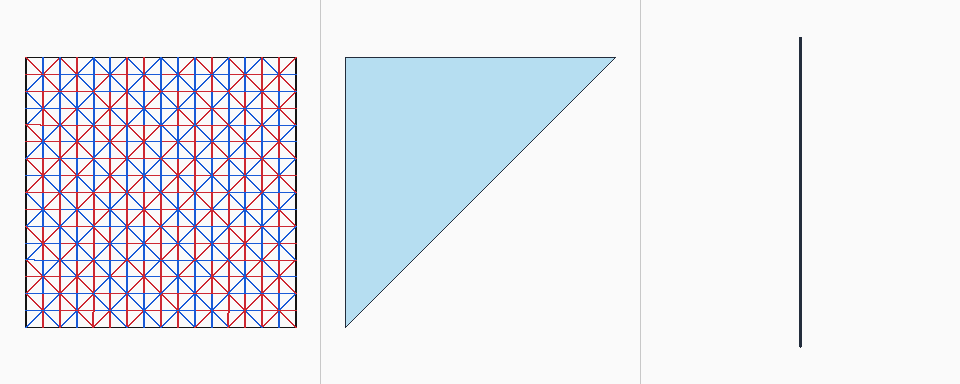
\includegraphics[width=\linewidth]{figures/dataset/sample-6.png}\par\medskip
}{
\noindent\fbox{\parbox{.9\linewidth}{Dataset gallery pending export: short all-layers,
longer all-layers, and some-layers examples.}}}
\IfFileExists{figures/dataset/sequences.tex}{\paragraph{all-layers/easy-0001 (all-layers, 4 reference folds)}
\noindent Stored state 0\par
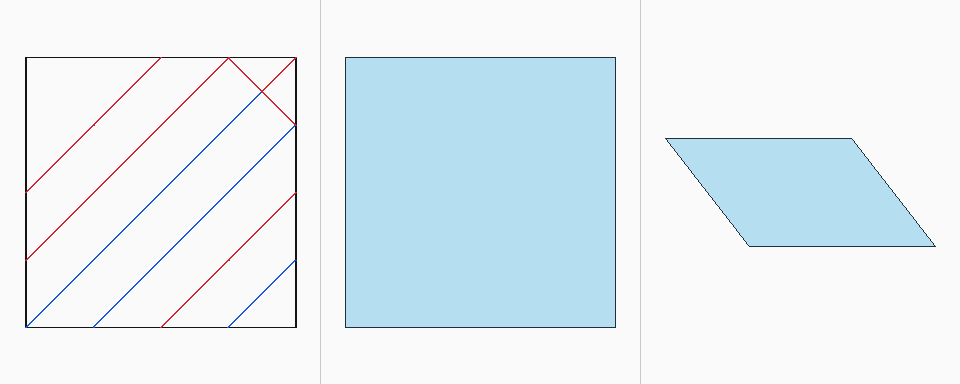
\includegraphics[width=.72\linewidth]{figures/dataset/sample-1-state-0.png}\par
\noindent Stored state 1\par
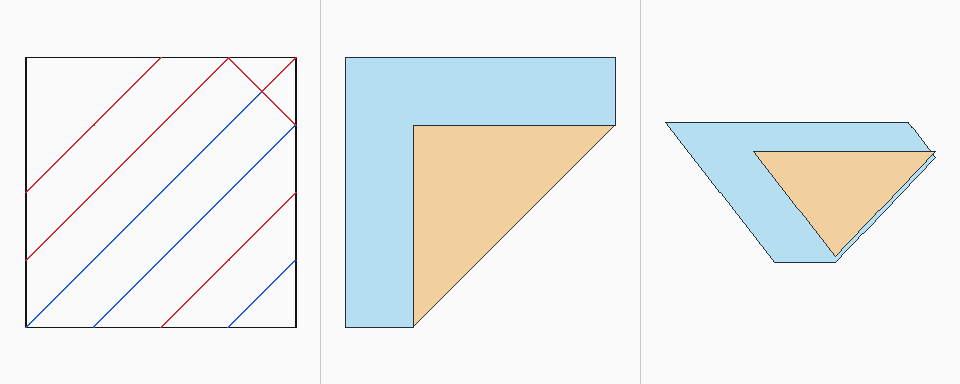
\includegraphics[width=.72\linewidth]{figures/dataset/sample-1-state-1.png}\par
\noindent Stored state 2\par
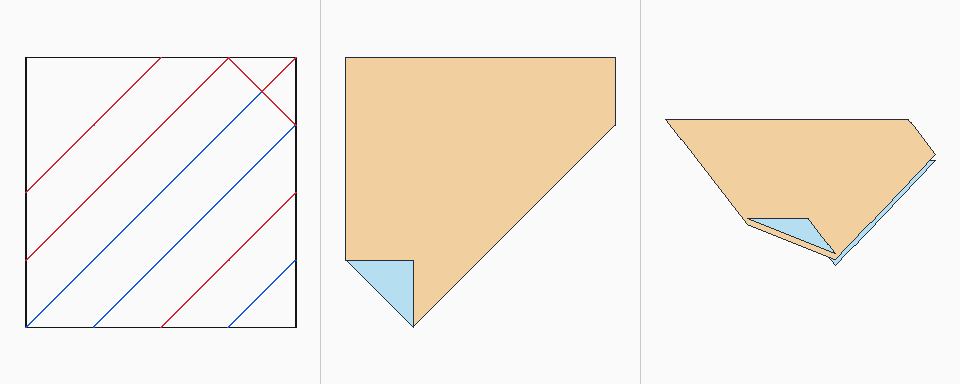
\includegraphics[width=.72\linewidth]{figures/dataset/sample-1-state-2.png}\par
\noindent Stored state 3\par
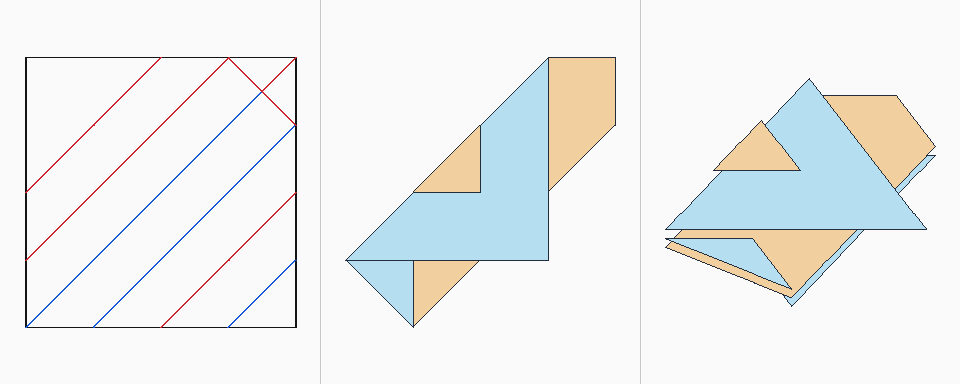
\includegraphics[width=.72\linewidth]{figures/dataset/sample-1-state-3.png}\par
\noindent Stored state 4\par
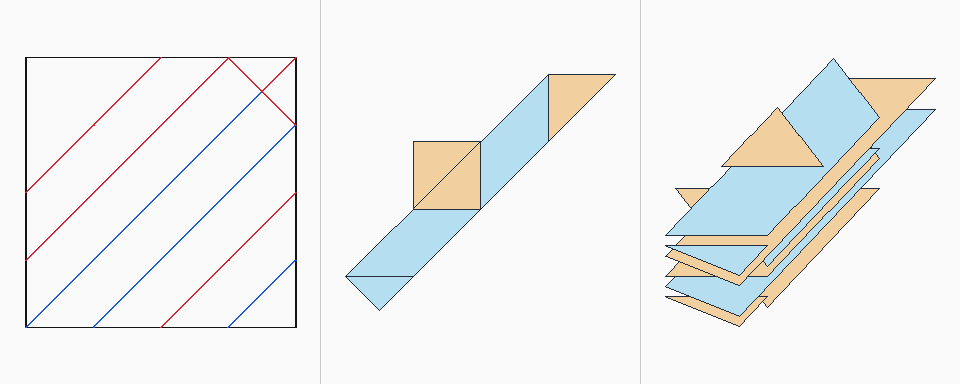
\includegraphics[width=.72\linewidth]{figures/dataset/sample-1-state-4.png}\par
\paragraph{all-layers/mid-0004 (all-layers, 11 reference folds)}
\noindent Stored state 0\par
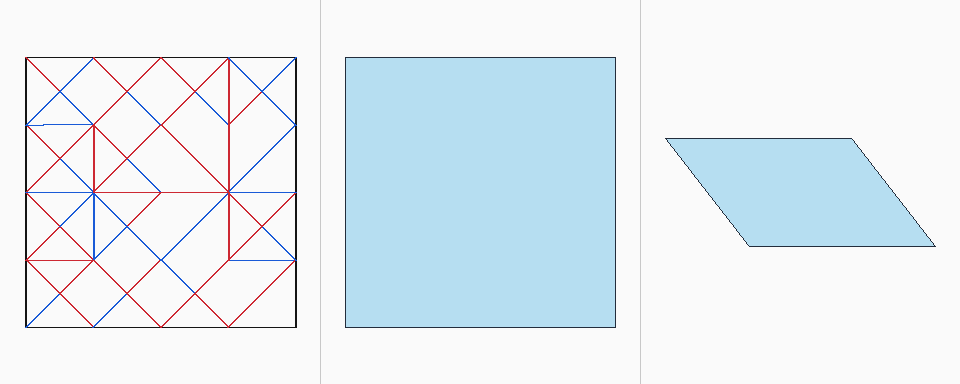
\includegraphics[width=.72\linewidth]{figures/dataset/sample-2-state-0.png}\par
\noindent Stored state 1\par
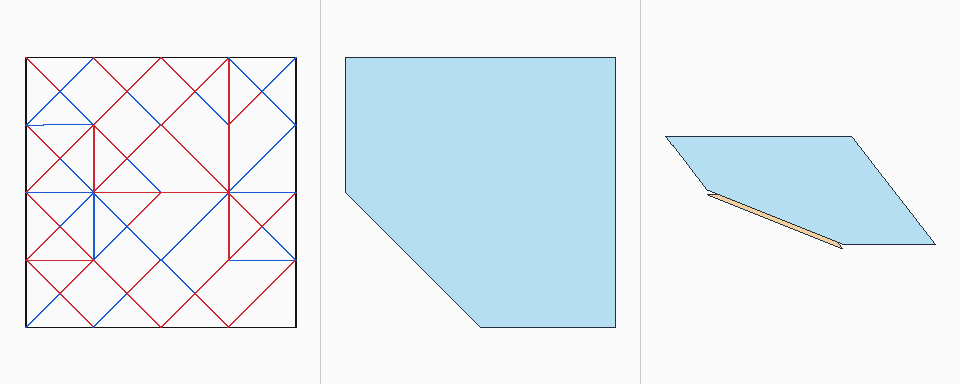
\includegraphics[width=.72\linewidth]{figures/dataset/sample-2-state-1.png}\par
\noindent Stored state 2\par
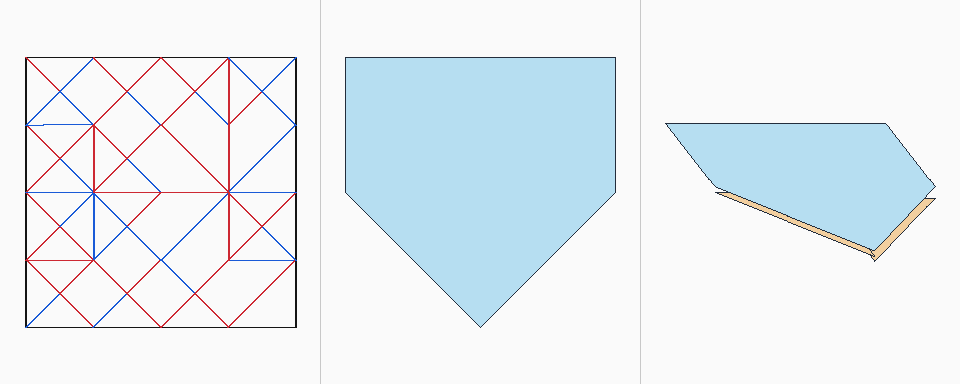
\includegraphics[width=.72\linewidth]{figures/dataset/sample-2-state-2.png}\par
\noindent Stored state 3\par
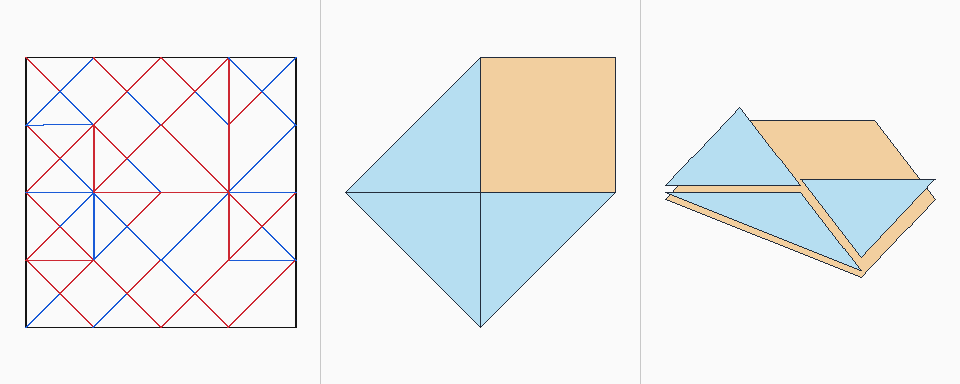
\includegraphics[width=.72\linewidth]{figures/dataset/sample-2-state-3.png}\par
\noindent Stored state 4\par
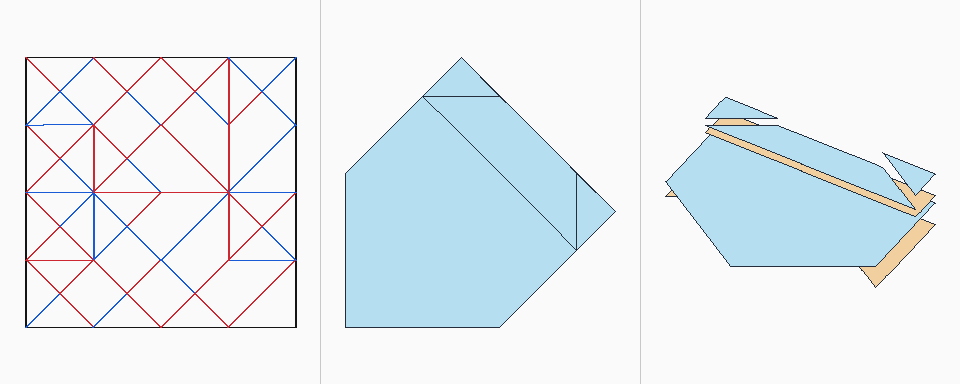
\includegraphics[width=.72\linewidth]{figures/dataset/sample-2-state-4.png}\par
\noindent Stored state 5\par
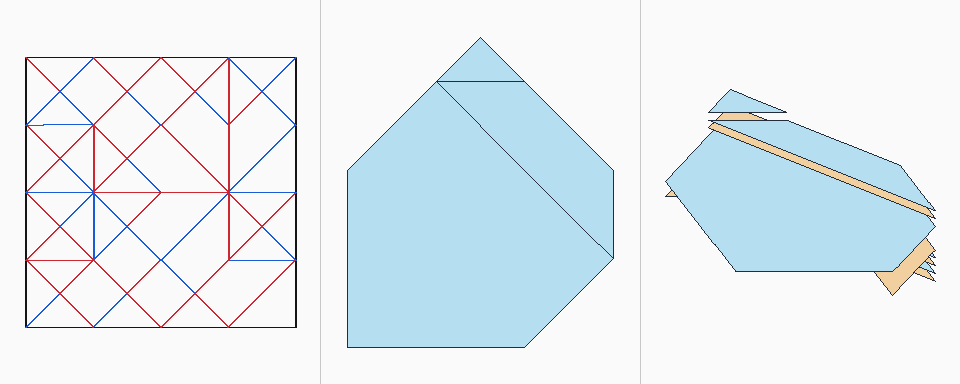
\includegraphics[width=.72\linewidth]{figures/dataset/sample-2-state-5.png}\par
\noindent Stored state 6\par
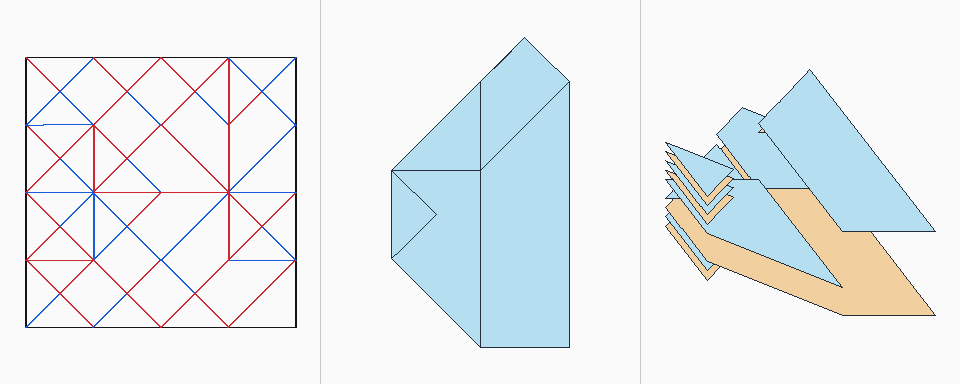
\includegraphics[width=.72\linewidth]{figures/dataset/sample-2-state-6.png}\par
\noindent Stored state 7\par
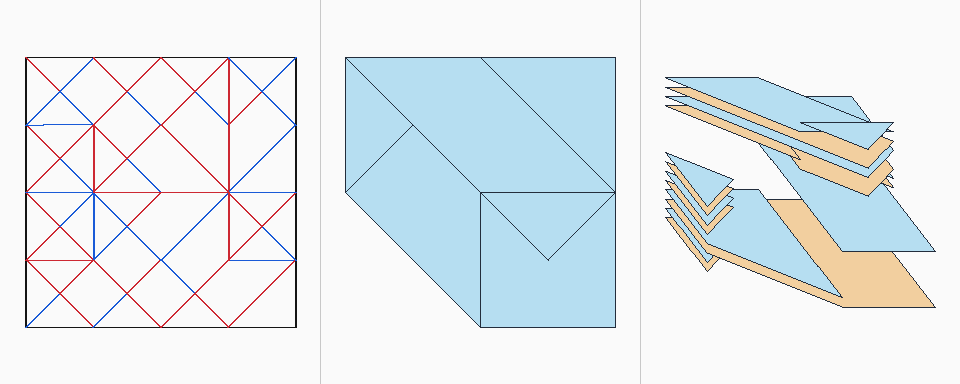
\includegraphics[width=.72\linewidth]{figures/dataset/sample-2-state-7.png}\par
\noindent Stored state 8\par
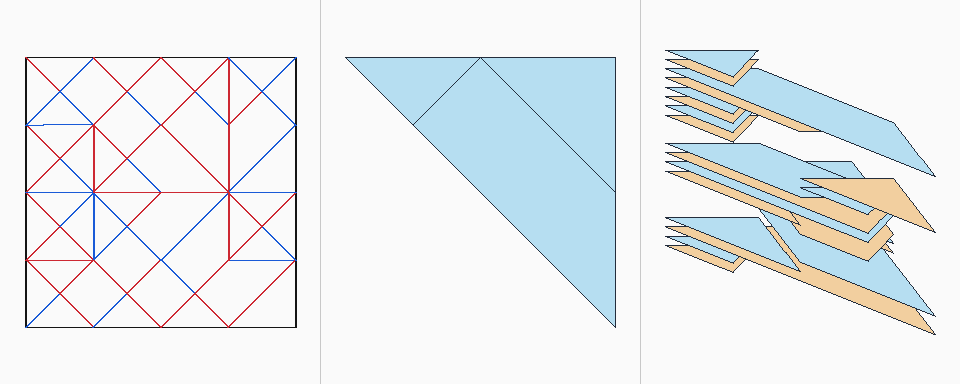
\includegraphics[width=.72\linewidth]{figures/dataset/sample-2-state-8.png}\par
\noindent Stored state 9\par
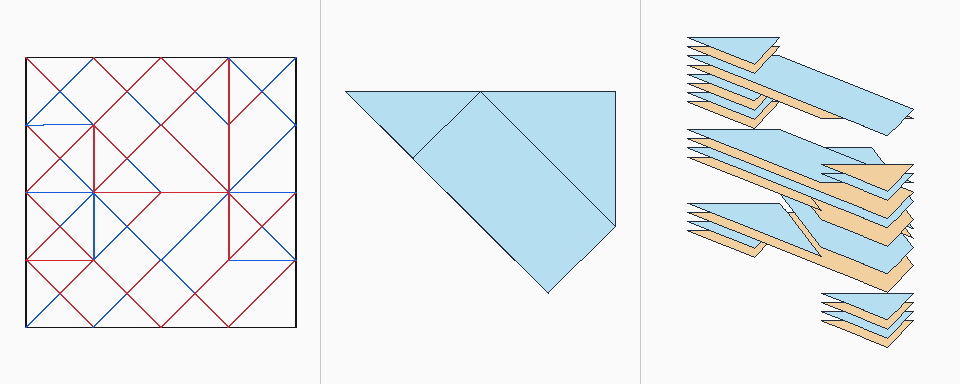
\includegraphics[width=.72\linewidth]{figures/dataset/sample-2-state-9.png}\par
\noindent Stored state 10\par
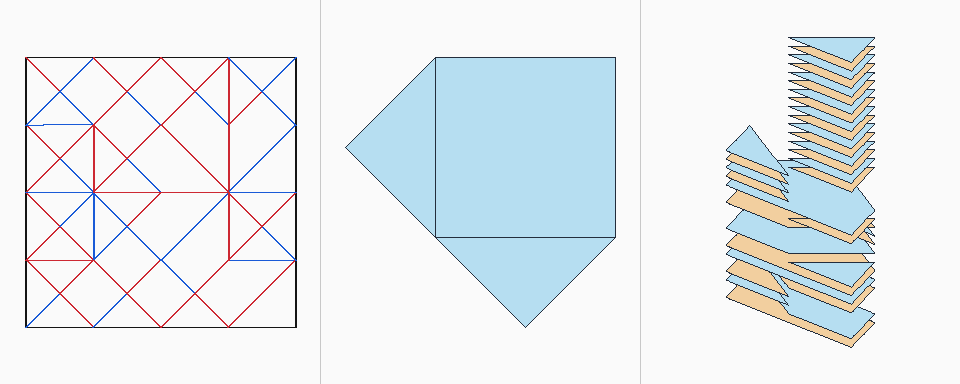
\includegraphics[width=.72\linewidth]{figures/dataset/sample-2-state-10.png}\par
\noindent Stored state 11\par
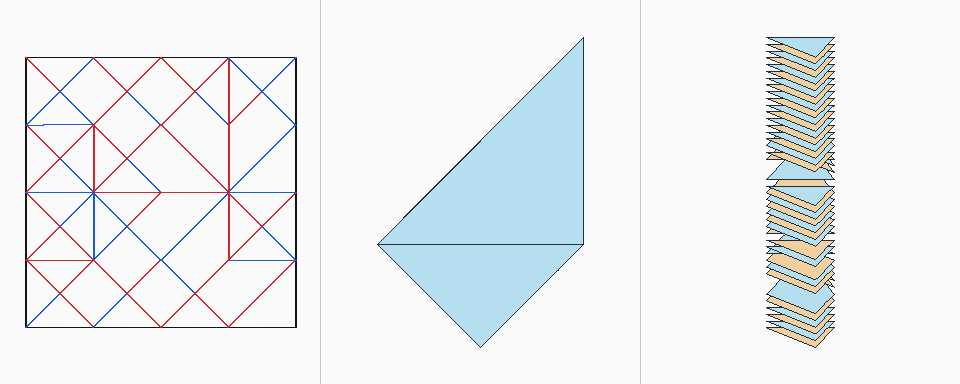
\includegraphics[width=.72\linewidth]{figures/dataset/sample-2-state-11.png}\par
\paragraph{some-generated-d5/layers-0001 (some-layers, 5 reference folds)}
\noindent Stored state 0\par
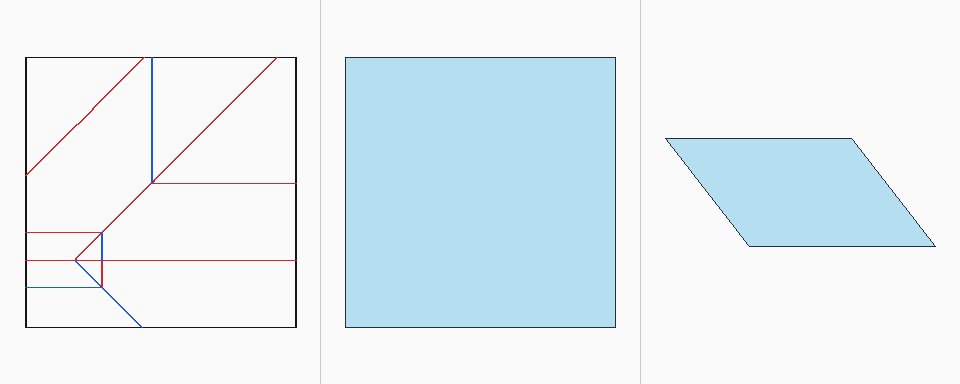
\includegraphics[width=.72\linewidth]{figures/dataset/sample-3-state-0.png}\par
\noindent Stored state 1\par
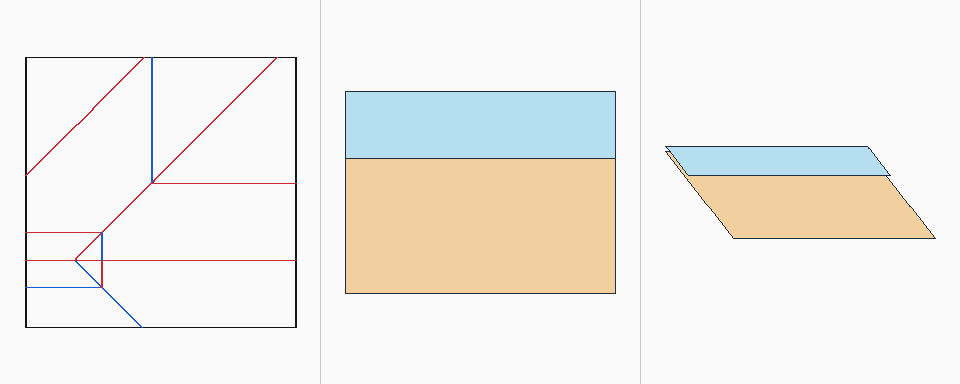
\includegraphics[width=.72\linewidth]{figures/dataset/sample-3-state-1.png}\par
\noindent Stored state 2\par
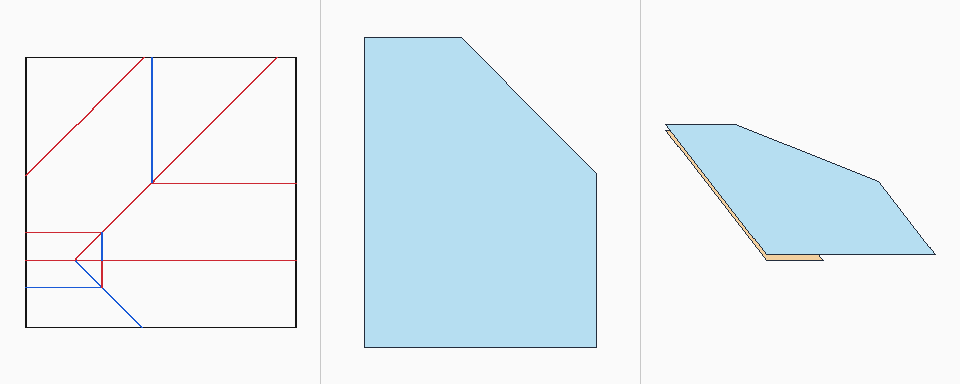
\includegraphics[width=.72\linewidth]{figures/dataset/sample-3-state-2.png}\par
\noindent Stored state 3\par
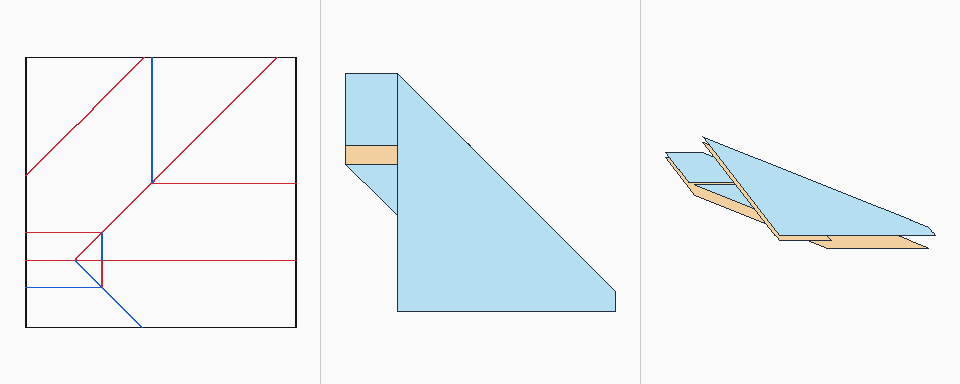
\includegraphics[width=.72\linewidth]{figures/dataset/sample-3-state-3.png}\par
\noindent Stored state 4\par
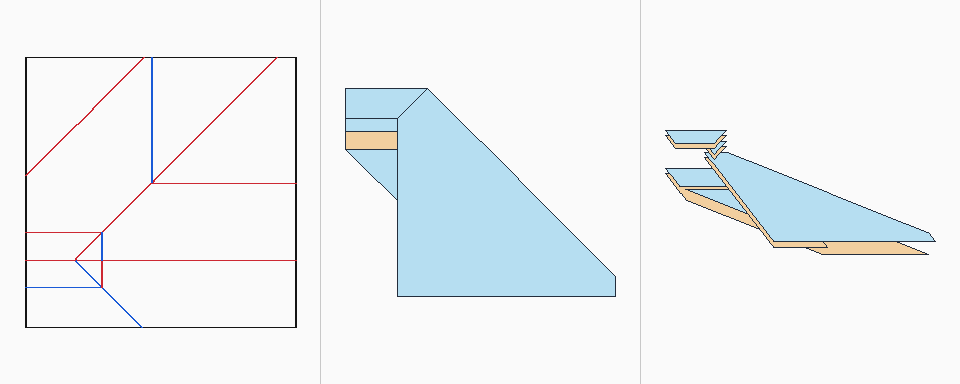
\includegraphics[width=.72\linewidth]{figures/dataset/sample-3-state-4.png}\par
\noindent Stored state 5\par
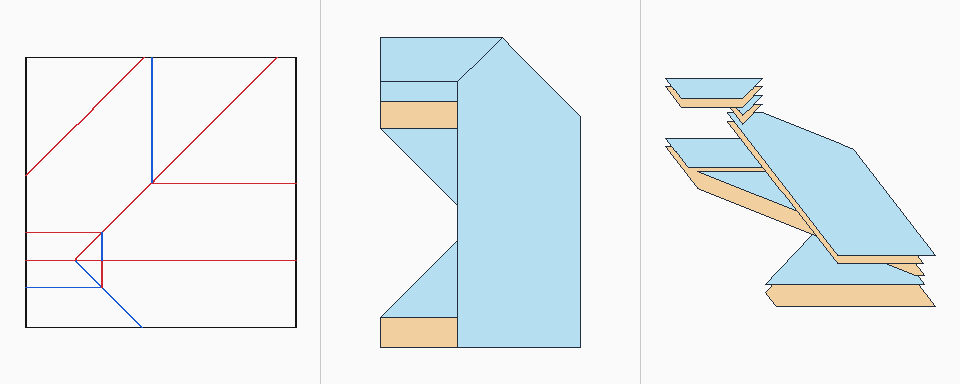
\includegraphics[width=.72\linewidth]{figures/dataset/sample-3-state-5.png}\par
}{}

\subsection{Trace-analysis interface}
We provide a trace-inspection interface for browsing saved runs, replaying recorded folding
trajectories, and examining model actions alongside tool feedback and rendered states. This
supports qualitative analysis of successful construction, repeated exploration, and unsuccessful
termination. A command-line trace viewer additionally supports filtering by task, trial,
session, role, and event type.

Figures~\ref{fig:dataset-browser-ui} and~\ref{fig:trace-viewer-ui} show the dataset
browser and trace viewer, respectively. These interfaces support inspection of
reference sequences and recorded model episodes.

\begin{figure}[tbp]
\centering

\includegraphics[width=\linewidth,height=.34\textheight,keepaspectratio]{\detokenize{../../assets/screenshots/Screenshot 2026-09-25 at 07.44.50.png}}
\caption{Dataset browser with \texttt{easy-0028} selected. The interface displays
sample metadata, the target crease pattern, and reference-sequence playback controls.
The right panel shows the unfolded sheet at step zero.}
\label{fig:dataset-browser-ui}
\end{figure}

\begin{figure}[tbp]
\centering

\includegraphics[width=\linewidth,height=.34\textheight,keepaspectratio]{\detokenize{../../assets/screenshots/Screenshot 2026-09-25 at 07.43.22.png}}
\caption{Trace viewer for a saved GPT-6 Luna attempt on \texttt{mid-0007}.
Run and turn navigation appear beside the current and target states. The selected
episode is marked unsolved; the displayed frame is at turn 12. Playback controls allow inspection of saved actions
and feedback.}
\label{fig:trace-viewer-ui}
\end{figure}

% EDITING NOTE: 07.44.33 is a second dataset-browser capture, not a verification
% capture; retained in assets/screenshots but omitted as redundant. Add an actual
% Verification-tab capture when available. Screenshots above are user-provided.

% EDITING NOTE: Select actual saved episodes after inspecting their terminal verdicts.
% Include one solved, one cycling, and one unsuccessful non-cycling attempt. For each,
% give run/sample IDs, configuration, terminal reason, and selected actions/tool responses.
% Include screenshots from traces.html: target/current state plus action and feedback panes.
% Include actual request/response excerpts; do not invent representative tool responses.
% Attach per-run budgets, effort, tool schemas, comparison tier, and supplementary results.

\subsection{Tool loading and configuration}
\label{app:tool-loading}
The schema builder selects the tools exposed in each run. Basic mode excludes candidate
enumeration; filtered mode includes it. Target comparison is added only when a comparison level
is configured. For an all-layers action model, partial-layer selection arguments are removed
from the exposed action schemas. The run configuration therefore records tool mode, comparison
level, and action model separately.

% REFUSAL FIGURE PLAN: Use a saved some-layers would-tear response with geometric diagnostics.
\subsection{Rejection feedback}
Figure~\ref{fig:rejection-feedback} illustrates the geometric evidence associated with
a \texttt{would-tear} response using the shared verification fixtures. The comparison
holds the initial state and hinge fixed and changes the selected layers. The export
script records both engine responses and checks that rejection preserves the state.
\begin{figure}[tbp]
\centering
\IfFileExists{figures/rejection-feedback-panels.tex}{
  \begin{minipage}[t]{.47\linewidth}
\centering
\textbf{(a) Rejected proposal}\par\smallskip
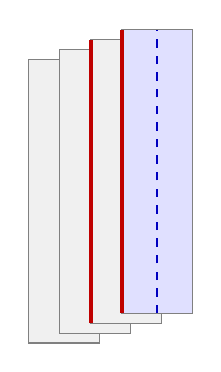
\begin{tikzpicture}[x=3.6cm,y=3.6cm,font=\scriptsize]
\draw[fill=gray!12,draw=gray] (0.000000,0.000000) -- (0.250000,0.000000) -- (0.250000,1.000000) -- (0.000000,1.000000) -- cycle;
\draw[fill=gray!12,draw=gray] (0.360000,0.035000) -- (0.110000,0.035000) -- (0.110000,1.035000) -- (0.360000,1.035000) -- cycle;
\draw[fill=gray!12,draw=gray] (0.220000,0.070000) -- (0.345000,0.070000) -- (0.470000,0.070000) -- (0.470000,1.070000) -- (0.345000,1.070000) -- (0.220000,1.070000) -- cycle;
\draw[fill=blue!12,draw=gray] (0.580000,0.105000) -- (0.455000,0.105000) -- (0.330000,0.105000) -- (0.330000,1.105000) -- (0.455000,1.105000) -- (0.580000,1.105000) -- cycle;
\draw[blue!75!black,dashed,thick] (0.455000,0.105000) -- (0.455000,1.105000);
\draw[red!75!black,line width=1.5pt] (0.330000,0.105000) -- (0.330000,1.105000);
\draw[red!75!black,line width=1.5pt] (0.220000,0.070000) -- (0.220000,1.070000);
\end{tikzpicture}\par
\texttt{would-tear}\par Top leaf selected; state unchanged.
\end{minipage}
\hfill
\begin{minipage}[t]{.47\linewidth}
\centering
\textbf{(b) Accepted proposal}\par\smallskip
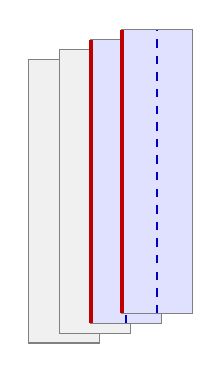
\begin{tikzpicture}[x=3.6cm,y=3.6cm,font=\scriptsize]
\draw[fill=gray!12,draw=gray] (0.000000,0.000000) -- (0.250000,0.000000) -- (0.250000,1.000000) -- (0.000000,1.000000) -- cycle;
\draw[fill=gray!12,draw=gray] (0.360000,0.035000) -- (0.110000,0.035000) -- (0.110000,1.035000) -- (0.360000,1.035000) -- cycle;
\draw[fill=blue!12,draw=gray] (0.220000,0.070000) -- (0.345000,0.070000) -- (0.470000,0.070000) -- (0.470000,1.070000) -- (0.345000,1.070000) -- (0.220000,1.070000) -- cycle;
\draw[blue!75!black,dashed,thick] (0.345000,0.070000) -- (0.345000,1.070000);
\draw[fill=blue!12,draw=gray] (0.580000,0.105000) -- (0.455000,0.105000) -- (0.330000,0.105000) -- (0.330000,1.105000) -- (0.455000,1.105000) -- (0.580000,1.105000) -- cycle;
\draw[blue!75!black,dashed,thick] (0.455000,0.105000) -- (0.455000,1.105000);
\draw[red!75!black,line width=1.5pt] (0.330000,0.105000) -- (0.330000,1.105000);
\draw[red!75!black,line width=1.5pt] (0.220000,0.070000) -- (0.220000,1.070000);
\end{tikzpicture}\par
\texttt{ok: true}\par Connected top pair selected.
\end{minipage}

}{
  \fbox{\parbox{.9\linewidth}{\small Rejection-feedback figure pending local export.
  The exporter checks rejected and accepted proposals from the same four-layer state
  before writing the panels and response evidence.}}
}
\caption{Rejection feedback and a legal alternative from the same state. Dashed blue
lines mark the proposed hinge; red segments mark the shared material edge identified
by the tearing diagnostic. Blue shading identifies selected layers. Selecting only
the top leaf would separate it from its connected neighbour away from the hinge;
selecting the connected top pair permits the fold. Both panels show the pre-action
state, with illustrative layer separation. The example is rendered from verification fixtures.}
\label{fig:rejection-feedback}
\end{figure}


\subsection{Protocol failure accounting}
\label{app:protocol-failures}
All 360 planned Luna ablation cases enter the solve-rate denominator. Of these,
355 have completed episodes. Two cases end at the request input-size limit:
\texttt{mid-0006} for GPT-5.6 Luna low with automatic feedback and GPT-6 Luna low
with legal enumeration. GPT-6 Luna low with legal enumeration on \texttt{mid-0010}
ends in a service prompt rejection. For GPT-6 Luna low with automatic feedback,
\texttt{mid-0006} and \texttt{mid-0010} were omitted from the restarted batch after
these blocking errors. These two cases are classified as omissions after blocking errors;
no direct service error is recorded for them in that condition. All five cases
count as unsuccessful evaluations under the planned protocol.

% Panel A: current stack, selected moving region, proposed hinge, and shared off-hinge edge.
% Panel B: original-sheet connectivity showing which moving/stationary regions share that edge.
% Label the rejection and note that the simulator retains the pre-action state.
% Do not render a torn state as an accepted simulation result. A counterfactual separation may
% be shown only as a clearly labelled explanatory schematic. Add a legal alternative only if
% the same-state action has been checked by the engine. Pending selection of a suitable trace.
